\documentclass[review]{elsarticle}

\usepackage{lineno,hyperref}
\modulolinenumbers[5]

\journal{Journal of \LaTeX\ Templates}

%%%%%%%%%%%%%%%%%%%%%%%
%% Elsevier bibliography styles
%%%%%%%%%%%%%%%%%%%%%%%
%% To change the style, put a % in front of the second line of the current style and
%% remove the % from the second line of the style you would like to use.
%%%%%%%%%%%%%%%%%%%%%%%

%% Numbered
%\bibliographystyle{model1-num-names}

%% Numbered without titles
%\bibliographystyle{model1a-num-names}

%% Harvard
%\bibliographystyle{model2-names.bst}\biboptions{authoryear}

%% Vancouver numbered
%\usepackage{numcompress}\bibliographystyle{model3-num-names}

%% Vancouver name/year
%\usepackage{numcompress}\bibliographystyle{model4-names}\biboptions{authoryear}

%% APA style
%\bibliographystyle{model5-names}\biboptions{authoryear}

%% AMA style
%\usepackage{numcompress}\bibliographystyle{model6-num-names}

%% `Elsevier LaTeX' style
\bibliographystyle{elsarticle-num}
%%%%%%%%%%%%%%%%%%%%%%%

\begin{document}

\begin{frontmatter}

\title{Examining Sentence Construction With An ACT-R Model of Language Production}
\tnotetext[mytitlenote]{Fully documented templates are available in the elsarticle package on \href{http://www.ctan.org/tex-archive/macros/latex/contrib/elsarticle}{CTAN}.}

%% Group authors per affiliation:
\author{Elsevier\fnref{myfootnote}}
\address{Radarweg 29, Amsterdam}
\fntext[myfootnote]{Since 1880.}

%% or include affiliations in footnotes:
\author[mymainaddress,mysecondaryaddress]{Elsevier Inc}
\ead[url]{www.elsevier.com}

\author[mysecondaryaddress]{Global Customer Service\corref{mycorrespondingauthor}}
\cortext[mycorrespondingauthor]{Corresponding author}
\ead{support@elsevier.com}

\address[mymainaddress]{1600 John F Kennedy Boulevard, Philadelphia}
\address[mysecondaryaddress]{360 Park Avenue South, New York}

\begin{abstract}
Our goal was to compare among different starting points in the process of language production. We accomplished this by building a model of language production that takes as input a set of words and attempts to construct a grammatical sentence from them. We pre-biased the model's initial utilities to start in the middle, beginning, and end of the sentence in order to add evidence to the debate of how incremental language production is. [Insert findings here]  Language production is an interesting process that is difficult to examine with traditional means. 
\end{abstract}

\begin{keyword}
language production\sep cognitive modelling
\MSC[2010] 00-01\sep  99-00
\end{keyword}

\end{frontmatter}

\linenumbers

\section{Introduction}
 How does the mind select words, sequence them, and produce sentences that communicate our intentions within context? The search for answers to this question has led researchers to a variety of models. Many models of psychology describe information processing and exchange; most linguistic models describe the representations that drive the process. The models explain empirical, qualitative observations; the fields have also developed quantitative metrics for evaluation. Obviously, models are underspecified in that they do not contain a computational (algorithmic) account that can carry out the process and predict testable effects. Specifically, a computational-psycholinguistic model of grammatical encoding has yet to emerge. The search for computational models that address related questions has been re-invigorated in recent years as large-scale language data have become available. This paper advances a computational cognitive model of grammatical encoding in language production by integrating work from somewhat separate fields. It uses a validated cognitive framework as well as broad-coverage grammars used by computational linguists, together with corpus-based evaluation techniques.
 
 This model is intended to be a starting point. Eventually, this model can help advance our understanding of language production by providing a unified model of several quite distinct effects. It will be quantitatively and architecturally plausible because it will be formulated within a cognitive framework, ACT-R (Newell, 1994; Anderson et al., 2004). This will make relationships between general cognition and memory and language processing clear. The model also uses insights from computational linguistics as it leverages a broad-coverage grammar formalism, CCG (Steedman, 2000). In this way, the model has the potential to advance theories in the field; however, it is presently only an advance in methodology. Similar models have been created to explain psycholinguistic theories as part of more general cognitive effects: for instance, syntactic priming as a product of cue-based memory retrieval \cite{priming-model}. 
 
However, while that model effectively explained one phenomenon, it could not produce the linguistic range found in corpora. Thus, more subtle linguistic phenomenon could not emerge. While explaining current data is required for any proposed model, the ultimate goal is prediction. A large range of possible models can explain all available data; however, by making testable predictions, a model can be validated beyond its peers.
 
\section{Motivation}
In the introduction to a volume reporting on the state of research in the field, psychologist Linda Wheeldon points out that language production “boasts a dedicated, imaginative, and highly productive group of researchers”, yet still lacks connection to other work, such as cognitive modeling. She also emphasized “the need for psychological models of language production to learn from theoretical linguistics in order to become better informed about the structure of language itself” (Wheeldon, 2000). A decade and a half later, researchers in computational psycholinguistics have dedicated themselves to the task of the interdisciplinary integration that Wheeldon called for. However, in language production, there is a need to combine the study of language, cognitive architecture, and linguistics.

Computational psycholinguistics has, in recent years, discovered a range of phenomena that may shape how we think about the mechanisms of human language acquisition and language processing. These phenomenon have origins ranging from information theory to learnability and have provoked important questions. As cognitive linguists ask ”How incremental is language production?” or ”How do people utilize working memory when realizing sentences?”, the boundaries are slowly being pushed for models to incorporate the full expressive range found in corpora. Meanwhile, while experiments have provided some answers to these questions, language production is particularly susceptible to experimental design. Without providing templates of some sort, such as \citet{sums-incr}\citet{prod-exp}, experimenters risk having too little data to answer their questions. However, providing templates eliminates an important piece of language production. Most critically, it is not yet clear if template selection is even a discrete step. If it is not, then by providing the template, it is possible that researchers are not simply eliminating one step from the task of language production but are changing the task to something else entirely. Thus, cognitive modelling is uniquely suited to answer questions when the design of the experiment moves the task too far from its naturalistic state. 

For example, consider an experimenter who wishes to contrast the choice of a Double Object construction (The boy threw his dog the ball) with a Prepositional Object construction (The boy threw the ball to his dog). If the participant is simply describing a picture, there is no guarantee he or she will even reference the dog! While these controls have been useful, they could have the side effect of muddling certain parts of the process: such as planning. In order to produce a sentence, it must first be planned. Investigating the planning process is difficult: many paradigms frequently used to investigate sentence comprehension, such as eye tracking or the visual world, seem much more difficult to apply. Despite the difficulty in designing experiments to measure planning, it is clearly of interest to researchers, as can be evidenced by ongoing debates. One such debate is to what degree is the process \emph{incremental}. 
 
For instance, with sentences that contain center-embedded clauses, is the end planned before or after the embedded clause? Consider the sentence "The dog that was chasing the cat that seemed to have rabies fell over." An incremental derivation would rely on \emph{surface order}: the actual order the words appear in the sentence. In other words, the speaker first plans "the dog", then "that was chasing the cat", then "that seemed to have rabies" and lastly "fell over." A less incremental derivation might be to plan "fell over" immediately after "the dog", and then to add the clauses later.
 
These questions are controversial, prompting ideas without clear cut answers. Due to the seeming difficulty in solving this debates such as these with more experimentation, we suggest turning to computational cognitive modeling, with a focus on models that are broad-coverage and can be empirically evaluated.
 
%
\section{Previous Work}
\subsection{Theories of Incrementality}


\subsection{Cognitive Models}
Language processing, in terms of both comprehension and production, have been explored broadly by the cognitive modeling community.

In terms of comprehension, cognitive models have been created both to explain several phenomenon and more generally. \citet{decision} explained the lexical decision task as a by-product of chunk activation. \citet{anaphoric} provides evidence that memory retrieval is likewise sufficient to explain whether nouns are treated as anaphoric: whether they refer to an antecedent or are a new reference. Both \citet{comp-model} and \citet{big-comprehension} make strides toward more general models of language comprehension.

The models to explain language production are thus far, more narrow. \citet{references} created a model that produced references for the iMAP task. \citet{model-priming} was a cognitive model of syntactic priming; it demonstrated that priming can be explained by activation. It made linguistic choices, but only well-defined choices, such as whether to choose double object or prepositional object constructions. 

While broader coverage models of language generation do exist \citep{chart}, they make no claims of cognitive plausibility. Thus, we see this paper as a step towards a broad, realistic model of language production. 
\section{Background}\label{sec:ccg}
Language comprehension could be briefly stated as the process of transforming words into meaning. Language production is the opposite process. Language production thus consists of several tasks, including transforming some semantic representation into words, and then combining those words into ideas. For now, we primarily focus on the second task, which we accomplish with a grammar formalism, \textit{Combinatory Categorial Grammar} (CCG) \citep{ccg}.

CCG is a grammar in the family of mildly-context sensitive grammars, along with Tree-Adjoining Grammar \citep{tag}. Mildly-context sensitive grammars have been shown to be capable of representing human speech, and computationally plausible in real-time \citep{convergence}. Also importantly, CCG stores only a single type value at any given point for combined words, as opposed to TAG which stores the entire tree. The types in CCG can be arbitrarily complex, but its rules are quite simple. See Figure~\ref{eqn:ccg} for a demonstration of the rules. See Figure~\ref{fig:ccg} for an example of a derivation.

\begin{figure}
\[X/Y > Y = X\]
\[Y < X\setminus Y = X\]
\[X/Y >> Y/Z = X/Z\]
\[Y\setminus Z << X\setminus Y = X\setminus Z\]
\caption{Forward Application, Backward Application, Forward Composition, and Backward Composition respectively. Note that types $A,B$ could be any of combinatorially derived types of CCG}
\label{eqn:ccg}
\end{figure}

\begin{figure}[ht]
\begin{center}
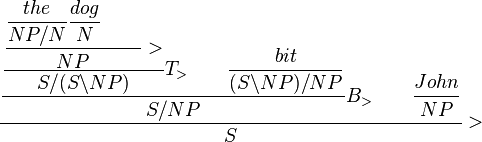
\includegraphics[width=0.95\columnwidth]{figures/ccg}
\end{center}
\caption{An example of a derivation of CCG. Note that the $T>$ is for type-raising, which is handled my declarative memory rather than production rules in my model. \textbf{Redo with my own application combinators}}  
\label{fig:ccg}
\end{figure}

\section{Model}
The presented model is implemented in jACT-R \citep{jactr}, a full Java implementation of the ACT-R theory \citep{actr}. Unlike other potential variants \citep{actup}, jACT-R has the same full set of constraints as ACT-R.  

The presented model's chunks and productions presently largely have a one to one correspondence with CCG. The primary production rules besides memory retrievals are rules directly from CCG; the primary computational units are the types in CCG.  

In theory, a model of language production should not make any more assumptions beyond ACT-R, in practice, the model relies on several simplifications. In the future, many of these could become parameters to a model to compare how well the model fits. The model's basic goal is to greedily combine lexical-syntactic chunks together to form a sentence. Right now, the process for that combination consists of the syntactic rules of CCG, and the model has no inherent preference for what to combine with what, besides as described later in experiments.

\subsection{Rules and Chunks}
The model itself, due to its ability to generalize to any sentence, is programatically generated. The model has \textit{classes} of rules and classes of chunks. A general layout of the production rules can be found in Figure~\ref{fig:prod}. The organizational scheme of the chunks can be found in Figure~\ref{fig:dm}.

\subsubsection{Production Rules}\label{sec:rules}
There are several classes of production rules. A class of production rules can be thought of as a type of operation, with each specific production rule being that operation on that chunk. For instance, it takes two separate production rules to combine two elements that are at different points in the sentence. Secondly, it takes a different production rule to determine which of the types the Lexsyn should use to combine. For instance, family can be either an adjective or a noun, and it could fill a slot earlier in the sentence ("My family and I went to eat dinner") or later ("I went with my family members to eat dinner"). The main classes of production rules are as follows:
\begin{itemize}
\item Move word $A$ into the model: The word moves from DM into the goal buffer. This class contains position information, so there are $N$ of them, where $N$ is the number of words in the sentence.
\item Retrieve lexsyn $A_{lex}$ for the word $A$: The type info moves from DM into the goal buffer. This class contains position information, so there are $N$ of them, where $N$ is the number of words in the sentence.
\item Apply Syntactic Rule to $A_{lex}$ and $B_{lex}$: CCG defines four basic and a few more complicated syntactic rules, which are described in Section~\ref{sec:ccg}. This class contains position and type information both two arguments, so there are $N * K * (N-1) * J$, where $N$ is the number of words in the sentence, $K$ is the number of types $A_{lex}$ has, and $J$ is the number of types $B_{lex}$ has
\item Resolve Syntactic Rule on $A_{lex}$: In this step, the new type that results from the previous operation is retrieved and stored in $A_{lex}$, and $B_{lex}$ is removed from the goal buffer.
\item Terminate and begin new sentence: If only a single lexsyn remains because all of them have been successfully combined, or no more rules are applicable, then the sentence is finished and the model will start its next goal. 
\end{itemize}

\subsubsection{Declarative Memory}\label{sec:dm}
Declarative Memory is composed of a few simple chunk types, described below.
\begin{itemize}
\item Word : A word simply has a name, which corresponds to its lexical information (e.g. family).
\item Type : A type is an arbitrarily complicated CCG type. The types that exist in DM are the types that are used in the Switchboard CCG derivations.
\item Lexsyn : A Lexsyn associates a Word with some number of Types. The chosen types are the types that the word has in the Switchboard corpus, including from type-raising.\footnote{Type-raising is a CCG operation where a type changes to a symbolically different but effectively equivalent type. This allows derivations in different orders.}
\item Sentence : A sentence is the work area to create the final utterance. Thus, it starts with words, which eventually become several Lexsyns, which eventually combine into a single Lexsyn, representing the finished sentence.
\end{itemize}

\begin{figure}[ht]
\begin{center}
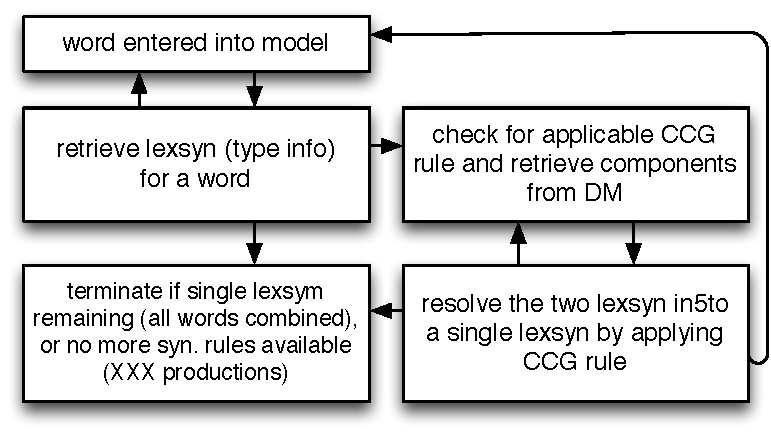
\includegraphics[width=0.95\columnwidth]{figures/model-FSA}
\end{center}
\caption{General process flow of the production rules of the model. See Section~\ref{sec:rules} for a more detailed description.}  
\label{fig:prod}
\end{figure}

\begin{figure}[ht]
\begin{center}
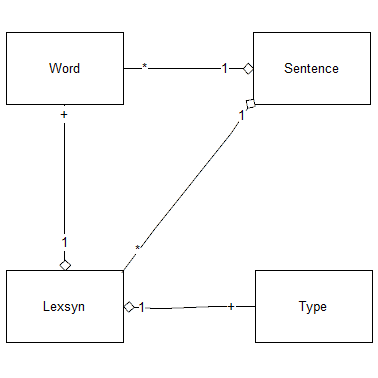
\includegraphics[width=0.95\columnwidth]{figures/prodtypes}
\end{center}
\caption{General data model of the declarative memory. See Section~\ref{sec:dm} for a more detailed description.}  
\label{fig:dm}
\end{figure}

\subsection{Input}
Normally, to simulate language production, we would prefer the model start with a semantic representation. Unfortunately, starting with a true semantic representation requires both an evaluation of that representation and an implementation of lexical selection. Thus, we used a simple proxy for the semantic representation as an unordered set of words that could create at least one valid sentence. The words are taken from sentences in the Switchboard corpus.

\subsection{Output}
The model attempts to produce a sentence. However, it does not always successfully finish a sentence, sometimes producing a fragment or several disconnected fragments.




\section{Methods}
While we use the bigram method previously described to evaluate the utterances described, we also need something to compare to. To do this, we put randomly sampled Switchboard sentences through the same evaluation scheme. We additionally compare variants of the model to this condition, to see which one best fits the data. As described earlier, our primary research question is to determine the degree that language production is incremental. We believe the effectiveness of each model in fitting the human data can provide evidence toward answering that question.

\begin{itemize}
\item The \textit{Incremental} model has an initial utility distribution that favors syntactic rules at the beginning of the sentence, decreasing for rules later in the sentence.
\item The \textit{Centered} model has an initial distribution favoring rules in the center of the sentence, decreasing as they get closer to the end and the beginning.
\item The \textit{Reverse} model has an initial distribution favoring rules at the end of the sentence, decreasing as they get closer to the beginning.
\item The \textit{Default} model has no initial utility distribution, with every rule starting at zero utility.
\end{itemize}

As a reminder, all of these utilities would change as the model progresses and makes sentences. However, the \textit{Default} model has certain disadvantages. As there is an initial sentence the model receives, having any imposed structure would make the model more likely to produce an utterance closer to that original sentence, which is presumably slightly more plausible than any given grammatical utterance. Nonetheless, we hypothesize due to a decreased cognitive load and an increased flexibility in the usage of syntactic rules that the \textit{Incremental} model will perform the best.

Each of the four models and the control condition were fed ten groups of one hundred sentences. Each of them is plotted and compared by their standard deviation, mean, and median.
%\section{Research Questions and Hypotheses}
We will investigate the likely start of sentence production by using a model that freely makes decisions. We do this by pre-biasing the utility of the versions of rules that are at various points in the sentence. We compare several initial utility distributions. 

\begin{itemize}
\item The \textit{Incremental} model has an initial utility distribution that favors syntactic rules at the beginning of the sentence, decreasing for rules later in the sentence.
\item The \textit{Centered} model has an initial distribution favoring rules in the center of the sentence, decreasing as they get closer to the end and the beginning.
\item The \textit{Reverse} model has an initial distribution favoring rules at the end of the sentence, decreasing as they get closer to the beginning.
\item The \textit{Control} model has no initial utility distribution, with every rule starting at zero utility.
\end{itemize}

As a reminder, all of these utilities would change as the model progresses and makes sentences. However, the \textit{Control} model has certain disadvantages. As there is an initial sentence the model receives, having any imposed structure would make the model more likely to produce an utterance closer to that original sentence, which is presumably slightly more plausible than any given grammatical utterance. Nonetheless, we hypothesize due to a decreased cognitive load and an increased flexibility in the usage of syntactic rules that the \textit{Incremental} model will perform the best.
%\section{DetailedModel}
\subsection{Chunks and Buffers}
Our model relies on a fairly simple set of chunks. 

\subsubsection{Word}
A word is the simplest type. It just has a name, which is the text of the word. It has no slots. The word chunks are built by creating a chunk of each word in the Switchboard corpus.

\subsubsection{Type}
At the heart of our model are chunks representing CCG syntactic types. There are two basic types of CCG types, though they appear to ACT-R as the same. One is what we refer to as a \textit{simple} type, where the type is a primitive type, such as a noun phrase. There are approximately ten basic CCG types found in the Switchboard data set. The second is a \textit{compound} type, where the type is composed of a left type, a right type, and a \textit{combinatory operator}. The left type and right type of each compound type can be either simple or additional compound types. Type chunks thus have three slots, the FullType, the LeftType, the RightType, and the Combinatory Operator (the last three are null if it is a simple type). Lastly, it has a flag to mark if that type is able to join (via conjunctions) with others of its type. The type chunks are built by creating a type for each type that appears in the Switchboard corpus.

\subsubsection{Combinatory Operator}
A combinatory operator is a very simple operator that can be thought of as a dependency within a type. As the end-goal of sentence production is to produce a sentence, a complete sentence is always of type \textit{S}, which is one of the CCG simple types. Then, verbs, adjectives, and so on are assigned compound types in such a way that they could ultimately be part of a complete sentence. For instance, an adjective might be NP/N, suggesting that it needs a noun to its right in order to be a noun phrase. If it was NP\textbackslash N, it would instead suggest it needs a noun to its left. Thus, the two combinatory operators are slash and backslash. Combinatory Operator chunks have no slots. These two combinatory operators are predefined.

\subsubsection{Lexsyn}
A Lexsyn is a Chunk that associates words with their type information. It, simply put, has a slot for the word, and then has the five slots for each type the word can take, where these slots are the exact same as described in the Type chunk. These are built by reading Switchboard, and associating every type (including type-raised types) that any given word ever takes with the word, and then creating the Lexsyn accordingly.  

\subsubsection{Sentence}
The Sentence is essentially the goal chunk. In this way, it basically contains predefined slots that are the input, and then predefined slots to store the output. Its first several slots is a set of words that are unordered. These are predefined, and consist of the words in a sentence that appears in Switchboard. The Sentence chunk also has several other slots, which correspond basically to lexsyns. Due to the methodology for accessing slots of slots, these are all stored in a flat manner, similarly to how the lexsyn stores types. Thus, the sentence chunk's total number of slots is the maximum number of words in the target sentences multiplied by the maximum number of types any given word has in the target sentences. This makes the chunk quite large. 

The final, correct output for the model is a single Lexsyn with the type S. In general, the output can be thought of as a Lexsyn that contains some number of words and some final syntactic type, where it can no longer combine with any of the other lexsyns. Details on how the Rules utilize the working space in the Sentence chunk will be covered in the next section. 

\subsection{Production Rules}
\subsubsection{Retrieving Syntactic Information}
There are two relevant production rules to begin processing: GrabWord and AddLexSyn. GrabWord is the simple process of retrieving syntactic information about a word in the input. It can fire at any time the retrieval buffer is not busy. This takes a word from the input and makes a retrieval request for a Lexsyn with that word. AddLexSyn then updates the goal state and does cleanup, by removing the word from input and adding the lexsyn to the goal buffer. This presently allows for an infinite working memory span, though the model in principle could work the same by having a fixed working memory span. As of now, however, this could possibly lead to retrieving a set of lexsyns where none could be combined. Both GrabWord and Lexsyn have as many variants as there are maximum number of words in a sentence. 

\subsubsection{Syntactic Rules and Resolutions}
Each Syntactic rule is defined many times, requiring dependencies in the Sentence chunk to be met. Mostly, this is by checking if any Lexsyns in the sentence chunk are matches for each other's dependencies. If it is a match, a retrieval request is put out for the matching type. This sets up another type of production rule to follow where the rule is resolved. This updates the type that's stored in chunk, removes the chunk that's been absorbed (in Composition, for no particular reason, the left always absorbs the right), and removes all other possible types of the new chunk, if they still exist. In other words, on the first combination, each Lexsyn contains multiple types, but after it's been combined and forms a type that's not specific to that word, the other types are removed as they are non-equivalent. The syntactic rules in CCG are described below. 

\begin{itemize}
\item \textit{Forward Application} is a simple combinatory rule where a single dependency of a compound type is resolved to the right (in other words, the type has the Slash combinatory operator). The type resolving the dependency can be a simple type or a compound type. 

\item \textit{Backward Application} is a simple combinatory rule where a single dependency of a compound type is resolved to the left (in other words, the type has the Backslash operator). The type resolving the dependency can be a simple type or a compound type.

\item \textit{Forward Composition} takes two compound types with the Slash operator. If one type has a dependency to the right, and the other type's left side resolves that dependency, then that type gains the other type's right side as a new dependency to the right but resolves its current one and adds that word to the right. 

\item \textit{Backward Composition} takes two compound types with the Backslash operator. If one type has a dependency to the left, and the other type's right side resolves that dependency, then that type gains the other type's left side as a new dependency to the left but resolves its current one and adds that word to the left.  

\item \textit{Begin Conjunction} corresponds to adding a conjunction to a type that could benefit from it. For instance, this would be the process of transforming "walking" to "and walking" or "walking and". 

\item \textit{Finish Conjunction} corresponds to adding an equivalent type to the phrase that contains the conjunction. In other words, it's the processing of transforming "and walking" to "talking and walking" or "walking and" to "walking and talking".
\end{itemize}
%\subsection{ACT-R}
ACT-R has a few basic units of organization. The primary units for declarative memory are \textit{chunks}. A chunk is a fairly simple concept that basically refers to one thing that can be retrieved or held in working memory. Chunks can be arbitrarily simple or complicated by way of \textit{slots}. A slot is a simple data type that corresponds to another chunk. The most primitive chunks thus have a name, but no slots. 

Buffers are a unit of cognition that can hold exactly one chunk. While ACT-R can, in theory, have an arbitrary number of buffers (including those such as the visual buffer or the auditory buffer), we make use of only the simplest buffers: the retrieval buffer and the goal buffer. The retrieval buffer can be thought of as the state of memory retrieval. It can be empty or it can be retrieving something or it can contain something it just retrieved. The goal buffer, on the other hand, can be thought of as working memory. It also can only contain one chunk, but it contains the state of the problem that is being solved. 

Production rules are the allowable manipulations of the buffers, and the conditions upon which those manipulations should be performed. For instance, a model could have a production rule that says to retrieve something when the goal buffer is at some state. It might, for instance, call for looking up the syntactic type of the word that's currently in a given slot in the goal buffer. These production rules, in combination with chunks, form a cognitive model of some task when by meeting these conditions iteratively, they can successfully transform the initial state of the problem into its goal state. 

ACT-R additionally has a couple of other mechanisms. One is a form of simple utility learning, where after a rule fires, it is rewarded, penalized, or neither. We will use this type of learning with the tracing model. Another is activation, which affects which matching chunk is retrieved. This activation can be used to explain many linguistic phenomenon, such as priming \citep{priming} \citep{model}.  

In the following, we'll present the full set of chunks and production rules that make up our model. 
%\subsection{Goals}
Our goal is to achieve this using the tight constraints of the ACT-R system \citep{actr}. We further attempt to stick within the constraints of plausibility by not relying on strategies such as resampling from previously heard input, due to its inability to produce novel productions. Instead, we define a range of operations that are defined in the Combinatory Categorial Grammar (CCG) \citep{ccg}, a minimally context sensitive grammar that is believed to be capable of all of the syntactic operations of human language \citep{convergence}. However, while our current system uses the operations of CCG, our theoretical basis of combinatory operations does not explicitly rely on CCG. Indeed, our system could in the future compare two combinatory systems for plausibility. Our longterm goals take nothing for granted: any operation, method, or structure that is cognitively plausible, fits the data, and produces realistic output is a possibility. 

In the short term, however, we make several assumptions about the operations and structure of language production. The model attempts to combine whatever words it wants, given its current settings, rules, chunks, and goals. It is natural for the model to make some mistakes, but it can still be compared with itself for \textit{plausibility}.

\subsection{Evaluation}
The model receives as input a set of words that made up a sentence in the Switchboard corpus. The model will then, using its knowledge about these words and possible combinatory operations, attempt to produce a sentence or sentence fragment. The goal is to be more plausible, though this is obviously somewhat difficult and controversial to measure. Our method was to average the bigram scores produced by the SRILM toolkit \citep{srilm} for a given sentence. We used the same method for evaluation as used by \citet{chart}. Then, we computed standard statistical metrics on the distribution of these scores: namely the mean, median, and standard error.

As the models are generating from the same bag of words, there should be no serious disadvantage to choosing uncommon but naturalistic phrases, especially over a large dataset. 
\section{Evaluation}
Naturally, while the model produces utterances, those utterances don't always make sense. Quantifying exactly what it is to make sense is obviously difficult, so we went with a simpler metric: what is probable. We scored each sentence using an ngram model using the SRILM toolkit trained on the BNC corpus \citep{srilm}. While we could have compared the utterance to the original sentence, since we are mostly bypassing the semantic representation component, we are more concerned with the model producing any good utterances, rather than the ones with the intended meaning. Obviously, the ngram score produced for any given sentence will vary depending on the content of that sentence; however, the distribution of the scores can still tell us how close each variant of the model is to actual human language. Naturally, ngram scores of human language do not follow a normal distribution, so simple statistics are not particularly useful. Instead, we turn to the wilcox test, which determines whether two sets of samples are from the same distribution. If certain conditions are indistinguishable from human language, while others are not, that would suggest something about that condition is more similar to human language. 

There are also more qualitative analyses we can do. An important feature of most cognitive processes is resource minimization. In other words, processes are trying to minimize memory usage, cognitive load, and realization time. Cognitive load is fairly difficult to measure using our process: it would depend, in part, when semantic ideas enter working memory, which is out of the scope of our current model's process. Realization time, depending largely on the length of the utterance, is also difficult to measure. However, memory usage just refers to the number of items in memory as the realization process proceeds. We defined every syntax node in memory as an item, and if two syntax nodes are joined, then so is the item in memory. While using working memory as an evaluation in of itself wouldn't show anything, if it corresponds to the other data, then it provides additional support for the methodology.

Also of interest is the correspondence between position in the sentence and the actual syntactic analysis of the result. Sentences are generally considered right-branching if they start with syntax nodes on the left, progressively adding syntax nodes to the right. Left-branching is the opposite: syntax nodes on the right are appended on the left. Obviously, sentences are not (in general) entirely right-branching or left-branching, but instead, a numerical value can be assigned to measure this. Our methodology was done by considering all subtrees: every subtree had some amount of left and right nodes, which are then tallied. A tree's right-branching score is the total number of nodes to the right divided by the total number of nodes to the left. Thus, a higher score means that the tree is more right-branching. We should expect this right-branching factor to correspond to the utility initializations, if the realizer is producing the same sentences as the original sentences. 

On the other hand, the utility initializations might not be teaching the realizer how to produce those same sentences, but something more fundamental about word order. It is possible, for instance, that certain phrases or syntactic category combinations are more likely to appear because of utility. To test this, we can actually compare the produced sentences to the target sentences, using a metric like edit distance. There are a few ways to measure edit distance, which would have different implications. For instance, if a slot-based approach is used, then phrases that are out of place would get no benefit. However, if a metric like Levenshtein distance is used, then it would take fewer moves to restore the original sentence if there are shared phrases. The correlations between these metrics and the others could inform us about the correct interpretation of our results.
\section{Results}
We evaluated approximately 650 sentences per condition. The basic statistics of the results are included in Table~\ref{stats}. It's unclear which of these statistics is the most important measure

\begin{table}
\centering
\begin{tabular}{l|ccc}
Condition & Mean & Median & Variance \\
Early & $10^{-5}$ & $10^{-11}$ & $10^{-7}$ \\ \hline
Middle & $10^{-7}$ & $10^{-11}$ & $10^{-11}$ \\
Late & $10^{-7}$ & $10^{-10}$ & $10^{-11}$ \\
Default & $10^{-7}$ & $10^{-10}$ & $10^{-11}$ \\
Control & $10^{-5}$ & $10^{-20}$ & $10^{-6}$ \\
\end{tabular}
\label{stats}
\caption{Recall that a higher probability means that those sentences are more likely. Due to the size of the numbers, only the order of magnitude is included.}
\end{table}

After confirming that the distributions were very far from normal, we proceeded with pairwise Wilcox tests, which can be seen in Table~\ref{result}.

\begin{table}
\centering
\begin{tabular}{l|cc}
Condition-Pair & w-score & p-value \\ \hline
Early-Default & 160050 & $<0.00001$ \\
Early-Control & 499320 & $<0.00001$ \\
Early-Middle & 2238700 & $0.1702$ \\
Early-Late & 177950 & $<0.00001$ \\
Middle-Late & 177950 & $<0.00001$ \\
Middle-Default & 161410 & $<0.00001$ \\
Middle-Control & 493680 & $<0.00001$ \\
Default-Late & 229670 & $0.0342$ \\
Default-Control & 541230 & $<0.00001$ \\
Late-Control & 545950 & $<0.00001$ 
\end{tabular}
\label{result}
\caption{The results of the pairwise Wilcox tests. The null hypothesis is that the two samples are drawn from the same distribution.}
\end{table}

The Wilcox test is determining what the probability is that two sets of samples could have been drawn from the same distribution. From this, we can conclude that the Early results are notably different than those for Default and Control. On the other hand, Early is not reliably different than Middle. The basic pattern of this suggests that there are three basic groups. Control is notably the best, which of course is not surprising, as it should be seen as an asymptote models hope to approach. Then, Early and Middle pattern together, while Default and Late pattern together. 

This of course, is fairly unsatisfying without some sort of ordering. It's impossible to get a perfectly valid comparison among statistics from this type of methodology; however, by looking at the simple statistics, we can vaguely conclude that Early is performing the best. Its values for mean, median, and variance are all closer to Control than the other conditions. Alternatively, we can look at the actual w-scores. While it is not intended to be used as a distance metric for distributions, a higher value means it's less probable the samples are from the same distribution. Along this metric, Early and Middle outperform Late and Default. 

\subsection{Branching Factor}
The branching factor, as explained earlier, could help pinpoint the exact difference between the conditions. In other words, since our analysis relied on a heuristic, measuring the branching factor of the sentences produced checks if they are measuring what we expect. If there was no systematic bias in sentence production, we would expect Early to be more right-branching, Late to be more left-branching, and Middle and Default to both be about even. 

Our process was fairly simple, looking at the order of combination and if left- or right-branching trees were being formed. An example tree is shown in Figure~\ref{tree}. The numbers represent the branching factors of each sub-tree. Branching factors are computed by weight: if a tree has more nodes in its left sub-tree, then it is more right-branching. The total branching factor is based on the sum of each of these subtrees. An alternative metric of branching factor just computes what percentage of branches are right-branching. This considers something right-branching if a larger tree to the left absorbs a smaller tree to the right. This naturally correlates very well with the previous metric. Both metrics per condition are displayed in Table~\ref{bfmem}. 

\subsection{Working Memory Load}
We expect a realistic process of sentence production to try to minimize cognitive load. We have an approximate measure of the working memory load from the trace of the process; however, it is important to recognize that it is fairly limited in its usefulness. While this does represent the memory of the syntactic process, it does not represent the memory of the semantic process. Typically, we assume a right-branching process will take less working memory, because semantic and lexical items can be retrieved as they are needed. However, in terms of syntax, a purely right-branching process and a purely left-branching process will take an equivalent amount of memory. This relationship can be fairly clearly displayed in Table~\ref{bfmem}. Nonetheless, we see an interesting phenomenon emerge, where the two cases that pattern together in ngram scores also pattern together in working memory load.

\begin{figure}[ht]
\begin{center}
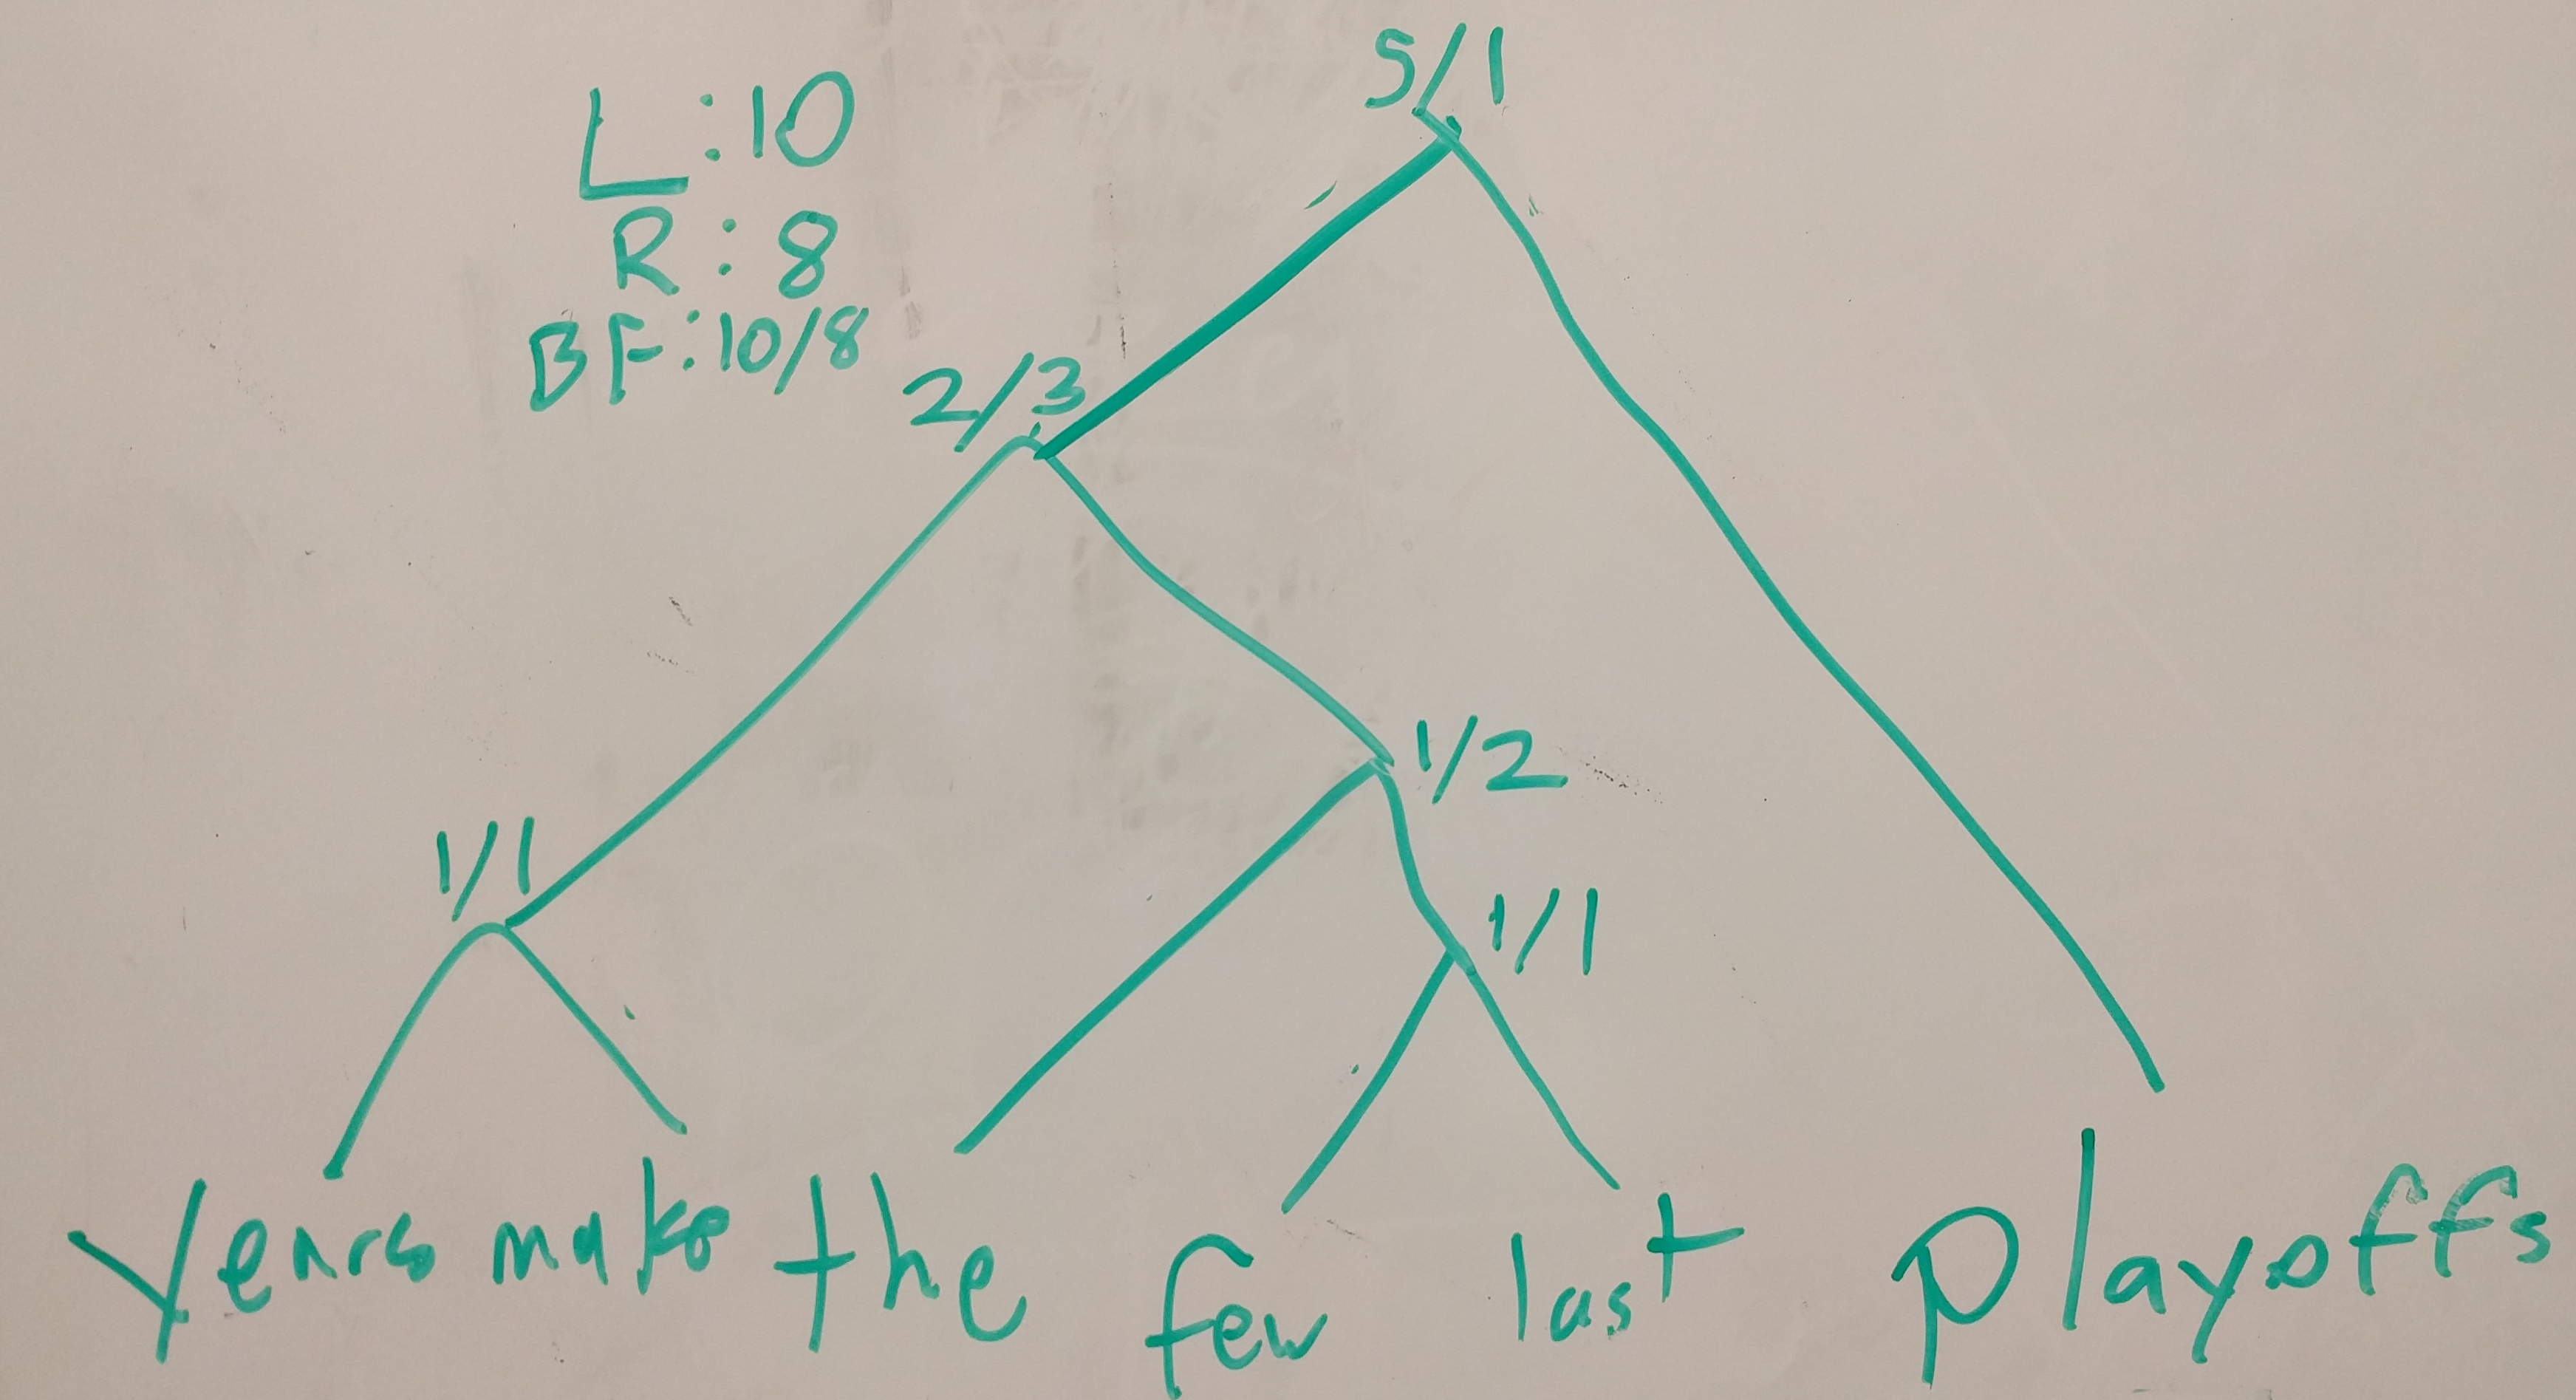
\includegraphics[width=0.95\columnwidth]{figures/tree}
\end{center}
\caption{An example of the syntax tree of actual output from the model. The overall branching factor of this tree is 10/8, or 1.25, indicating that it is primarily right-branching. This means that this tree represents a more incremental process.\textbf{temp diagram}}  
\label{tree}
\end{figure}

\begin{table}
\centering
\begin{tabular}{l|cccc}
Condition & RBF & RBF-alt & WM-eff & WM-avg \\ \hline
Early & 0.811 & 0.065 & 1.931 & 2.915 \\
Middle & 1.276 & 0.283 & 1.964 & 2.926 \\
Late & 1.102 & 0.165 & 1.654 & 3.112 \\
Default & 1.124 & 0.164 & 1.646 & 3.255 \\
\end{tabular}
\label{bfmem}
\caption{RBF and RBF-alt refer to the right-branching factor. In both, higher numbers means more right-branches. WM-eff is the average size of sentence produced per working memory used, so higher is better. WM-avg is just how much space is used, so lower is better.}
\end{table}

\subsection{Edit Distance}
Edit distance reflects how closely the model recreated the original sentence. While this is not necessarily the exact goal, it possibly reflects the strategy the models are using to perform better than the others. Further, while our semantic representation is weak, edit distance is a generally good metric to measure performance, as it relates all parts of the realization process. The specific edit distance metric we used is Levenshtein distance, which, due to its flexibility, will less strongly penalize phrases that are misplaced. This means that a low Levenshtein distance could suggest that a model is learning something about word order. Additionally, we looked at what we refer to as \textit{slot-based} edit distance. This simple metric just penalizes a sentence for each time it does not exactly match the input sentence. Lastly, we used the ROUGE metric, a metric originally designed for paraphrase similarity that can be thought of as a metric of semantic similarity \citep{rouge}. ROUGE has three measurements, based on shared ngrams, shared skipgrams, and shared subsequences, respectively. The results of these metrics can be seen in Table~\ref{distance}. 

\begin{table}
\centering
\begin{tabular}{l|ccccc}
Condition & Slot-Based & Leven & ROUGE-N & ROUGE-L & ROUGE-S  \\ \hline
Early & 0.811 & 0.065 & 0.028 & 0.036 & 0.000 \\
Middle & 1.276 & 0.283 & 0.029 & 0.039 & 0.004 \\
Late & 1.102 & 0.165 & 0.017 & 0.031 & 0.003 \\
Default & 1.124 & 0.164 & 0.016 & 0.024 & 0.000 \\
\end{tabular}
\label{distance}
\end{table}
\section{Discussion}
There is some amount of convergence in the performance based metrics. Middle and Early seem to do the best. Interestingly, this correlates very well with reduced memory. Problematically, our measure of memory is somewhat incomplete. 

Also from the metrics, we can glean that Middle seems to be using a mostly incremental process, while Early seems to be using the exact opposite. While it's not entirely clear while our condition would cause that, the penalty is substantially reduced, as the model is not presently measured on the semantic information it has to store. 

While models like this have no formal system of evaluation, we take the vague convergence of many metrics to be a sign of success for the modeling paradigm.
\section{Conclusion}
In this paper, we presented a methodology for pursuing psycholinguistic research. Borrowing from linguistic theory and computational modeling, we discussed how cognitive models, such as those implemented in ACT-R, can move beyond hand-coded models and pre-determined datasets. Further, we discuss how our model can disentangle somewhat complicated phenomena due to the ease with which several important variables, such as the capacity of working memory, can be manipulated. In particular, we find that sentences that require less working memory are easier to realize, but that having additional working memory available improves overall performance. We further find that performance increases as sentences are more right-branching, which we see as in line with previous research.
%\section{Chunks and Buffers in the Model}
Our model relies on a fairly simple set of chunks. 

\subsection{Word}
A word is the simplest type. It just has a name, which is the text of the word. It has no slots. The word chunks are built by creating a chunk of each word in the Switchboard corpus.

\subsection{Type}
At the heart of our model are chunks representing CCG syntactic types. There are two basic types of CCG types, though they appear to ACT-R as the same. One is what we refer to as a \textit{simple} type, where the type is a primitive type, such as a noun phrase. There are approximately ten basic CCG types found in the Switchboard data set. The second is a \textit{compound} type, where the type is composed of a left type, a right type, and a \textit{combinatory operator}. The left type and right type of each compound type can be either simple or additional compound types. Type chunks thus have three slots, the FullType, the LeftType, the RightType, and the Combinatory Operator (the last three are null if it is a simple type). Lastly, it has a flag to mark if that type is able to join (via conjunctions) with others of its type. The type chunks are built by creating a type for each type that appears in the Switchboard corpus.

\subsection{Combinatory Operator}
A combinatory operator is a very simple operator that can be thought of as a dependency within a type. As the end-goal of sentence production is to produce a sentence, a complete sentence is always of type \textit{S}, which is one of the CCG simple types. Then, verbs, adjectives, and so on are assigned compound types in such a way that they could ultimately be part of a complete sentence. For instance, an adjective might be NP/N, suggesting that it needs a noun to its right in order to be a noun phrase. If it was NP\textbackslash N, it would instead suggest it needs a noun to its left. Thus, the two combinatory operators are slash and backslash. Combinatory Operator chunks have no slots. These two combinatory operators are predefined.

\subsection{Lexsyn}
A Lexsyn is a Chunk that associates words with their type information. It, simply put, has a slot for the word, and then has the five slots for each type the word can take, where these slots are the exact same as described in the Type chunk. These are built by reading Switchboard, and associating every type (including type-raised types) that any given word ever takes with the word, and then creating the Lexsyn accordingly.  

\subsection{Sentence}
The Sentence is essentially the goal chunk. In this way, it basically contains predefined slots that are the input, and then predefined slots to store the output. Its first several slots is a set of words that are unordered. These are predefined, and consist of the words in a sentence that appears in Switchboard. The Sentence chunk also has several other slots, which correspond basically to lexsyns. Due to the methodology for accessing slots of slots, these are all stored in a flat manner, similarly to how the lexsyn stores types. Thus, the sentence chunk's total number of slots is the maximum number of words in the target sentences multiplied by the maximum number of types any given word has in the target sentences. This makes the chunk quite large. 

The final, correct output for the model is a single Lexsyn with the type S. In general, the output can be thought of as a Lexsyn that contains some number of words and some final syntactic type, where it can no longer combine with any of the other lexsyns. Details on how the Rules utilize the working space in the Sentence chunk will be covered in the next section. 

%\section{Production Rules}
\subsection{Retrieving Syntactic Information}
There are two relevant production rules to begin processing: GrabWord and AddLexSyn. GrabWord is the simple process of retrieving syntactic information about a word in the input. It can fire at any time the retrieval buffer is not busy. This takes a word from the input and makes a retrieval request for a Lexsyn with that word. AddLexSyn then updates the goal state and does cleanup, by removing the word from input and adding the lexsyn to the goal buffer. This presently allows for an infinite working memory span, though the model in principle could work the same by having a fixed working memory span. As of now, however, this could possibly lead to retrieving a set of lexsyns where none could be combined. Both GrabWord and Lexsyn have as many variants as there are maximum number of words in a sentence. 

\subsection{Syntactic Rules and Resolutions}
Each Syntactic rule is defined many times, requiring dependencies in the Sentence chunk to be met. Mostly, this is by checking if any Lexsyns in the sentence chunk are matches for each other's dependencies. If it is a match, a retrieval request is put out for the matching type. This sets up another type of production rule to follow where the rule is resolved. This updates the type that's stored in chunk, removes the chunk that's been absorbed (in Composition, for no particular reason, the left always absorbs the right), and removes all other possible types of the new chunk, if they still exist. In other words, on the first combination, each Lexsyn contains multiple types, but after it's been combined and forms a type that's not specific to that word, the other types are removed as they are non-equivalent. The syntactic rules in CCG are described below. 

\subsubsection{Forward Application}
Forward Application is a simple combinatory rule where a single dependency of a compound type is resolved to the right (in other words, the type has the Slash combinatory operator). The type resolving the dependency can be a simple type or a compound type. 
\subsubsection{Backward Application}
Backward Application is a simple combinatory rule where a single dependency of a compound type is resolved to the left (in other words, the type has the Backslash operator). The type resolving the dependency can be a simple type or a compound type.
\subsubsection{Forward Composition}
Forward Composition takes two compound types with the Slash operator. If one type has a dependency to the right, and the other type's left side resolves that dependency, then that type gains the other type's right side as a new dependency to the right but resolves its current one and adds that word to the right. 
\subsubsection{Backward Composition}
Backward Composition takes two compound types with the Backslash operator. If one type has a dependency to the left, and the other type's right side resolves that dependency, then that type gains the other type's left side as a new dependency to the left but resolves its current one and adds that word to the left.  
\subsubsection{BeginConjunction}
This corresponds to adding a conjunction to a type that could benefit from it. For instance, this would be the process of transforming "walking" to "and walking" or "walking and". 
\subsubsection{FinishConjunction}
This corresponds to adding an equivalent type to the phrase that contains the conjunction. In other words, it's the processing of transforming "and walking" to "talking and walking" or "walking and" to "walking and talking".

%\section{Research Questions}
\subsection{Starting Point of Sentence Production}
We will investigate the likely start of sentence production by using the naturalistic model. We will do this by pre-biasing the utility of the versions of rules that are at various points in the sentence. We could compare several initial utility distributions. As explained earlier, we could then compare the sentence or sentence fragments on the basis of their ngram scores.

\subsection{Incremental or Non-Incremental Production}
We have both an incremental CCG derivation and a normal form CCG derivation of the switchboard corpus. In this way, our model tracer's selection of what rule is \textit{correct} is really choosing from a set of rules, and it's using a derivation in order to guide it. However, at any given point, these derivations will have different rules that are correct or incorrect. By adjusting the model tracer, we can compare using the tracer model which of these derivations is more learnable.  

\subsection{Other Ideas}
The organization of the types for any given lexsyn and their initial utilities could also be investigated using a similar method as the starting point. For instance, with some uniform organization, we could investigate any number of questions, such as whether it is easier to start sentences with nouns.
%\section{Conclusion}
In this paper, we have presented an ACT-R model of language production capable of producing novel sentences and sentence fragments. It takes as input a set of words, having foreknowledge of both a larger set of words and the syntactic types those words can be. Then, it attempts to combine these words using the rules defined in CCG. The model has two modes, one where errors are measured over time (learnability) as the model attempts to produce a sentence that exists in the Switchboard corpus, and another where the plausibility of whatever the model did produce is measured. This allows us to ask a variety of interesting scientific questions of the model that previous studies have been unable to answer.

\section*{References}
\bibliography{lang, gen, models}

\end{document}